\documentclass[12pt]{article}

\usepackage{pablo-devoir}
\usepackage{pablo-listings}
\usepackage[a5paper,margin=1.5cm]{geometry}

\pagestyle{empty}

\title{Rep\'erage}
\date{1\up{er} octobre}
\classe{2\up{des}14}
\dsnum{DS 1}

\begin{document}

\maketitle

\begin{exercice}[Intervalles --- 3 points]
Résoudre le couple d'inéquations suivant, et représenter l'ensemble des solutions sur la droite des réels, puis sous forme d'intervalle.
\[\frac{x}{2}+1\geq5 \text{ et } 5-x>-8\]
\end{exercice}

\begin{exercice}[Coordonnées --- 3 points]
On considère la figure suivante, où $BCGH$ est un rectangle, et $EFCD$ est un carré. Répondre aux questions suivantes par lecture graphique.

\begin{multicols}{2}

\begin{center}
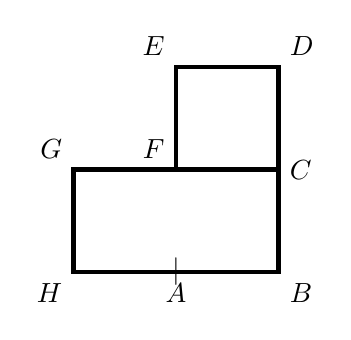
\begin{tikzpicture}[scale=1.3,ultra thick]
  \coordinate (A) at (1,0);
  \coordinate (B) at (2,0);
  \coordinate (C) at (2,1);
  \coordinate (D) at (2,2);
  \coordinate (E) at (1,2);
  \coordinate (F) at (1,1);
  \coordinate (G) at (0,1);
  \coordinate (H) at (0,0);

  \draw (H) node[below left]{$H$}
     -- (B) node[below right]{$B$}
     -- (C) node[right]{$C$}
     -- (G) node[above left]{$G$}
     -- cycle;
  \draw (A) node{$|$} node[below]{$A$};   
  \draw (C) 
     -- (D) node[above right]{$D$}
     -- (E) node[above left]{$E$}
     -- (F) node[above left]{$F$};

\end{tikzpicture}
\end{center}


\begin{enumerate}[(a)]
  \item Dans le repère $(A, B, F)$, quels points ont pour coordonnées $(-1;0)$ et $(1; 1)$ ?
  \item Quelles sont les coordonnées de $C$ dans le repère $(H, B, G)$ ?
\end{enumerate}
\end{multicols}

\end{exercice}

\begin{exercice}[Problème --- 11 points]
\emph{On rappelle que les réponses par lecture graphique ne seront pas acceptées.}
\begin{enumerate}[(a)]
  \item Dans un repère orthonormé, placer les points $A(2;0)$, $B(-0,5;0)$ et $C(1;2)$.
  \item Montrer que le triangle $ABC$ est isocèle en $B$.
  \item Calculer les coordonnées de $I$, milieu de $\left[AC\right]$.
  \item Calculer les coordonnées de $D$, symétrique de $B$ par rapport à $I$.
  \item Montrer que $ABCD$ est un parallélogramme.
  \item Peut-on être plus précis sur la nature de $ABCD$ ?
\end{enumerate}
\end{exercice}

\pagebreak

\begin{exercice}[Algorithmique -- 3 points]
  Dans un repère orthonormé, on considère le cercle $\mathcal{C}$ de centre $A(1, 0)$ et de rayon 5.
  \begin{enumerate}[(a)]
    \item Soit $B(3;5)$. Calculer la longueur $AB$. Le point $B$ appartient-il au cercle $\mathcal{C}$ ?
    \item Compléter l'algorithme suivante, pour qu'étant données les coordonnées d'un point du plan, il détermine si oui ou non ce point fait partie du cercle $\mathcal{C}$.
  \end{enumerate}

  \begin{lstlisting}[language=naturel,frame=lines,mathescape=true]
  Lire x
  Lire y
  Si $\ldots$
  Alors
    Afficher "Le point appartient au cercle $\mathcal{C}$"
  Sinon
    $\ldots$
  FinSi
  \end{lstlisting}

\end{exercice}

\begin{exercice}[Bonus --- 0,5 points + 0,5 points pour l'originalité]
Citer un mathématicien, et dire pourquoi il est connu.
\end{exercice}
\end{document}
